\chapter{Teorie} \label{sec:Teorie}

V této kapitole je shrntu teorie a sepsány potřebné informace pro realizaci a pochopení výstupů práce. Jsou popisovány zejména problematiky z oboru \acs{MIR} popsaném v bodě \ref{sec:MIR}. Metodz pro extrakci parametrů z hudebních nahrávek a principy pro pochopení jak tyto metody fungují. Poslední bod \ref{sec:Spectoda} této kapitoly je zaměřen na systém Spectoda jeho možnosti tvorby interaktivních světelných animací a ovládání světelných zdrojů. 

\section{MIR - Music information retrieval} \label{sec:MIR}
    Music information retrieval je interdisciplinární vědní obor soustředící se na získávání infromací z hudebních nahrávek.
    Jsou zde kombinovány znalosti mnoha oborů jako jsou muzikologie, psychoakustika, strojové učení, zpracování signálů a další. 
    
    Výstupy jeho výzkumu jsou využívány v populárních technologických aplikacích. 
    Jednou z aplikací je personalizované doporučování hudebních skladeb, které se nachází v moderních streamovacích platformách.
    Další využítí je v programech pro mixování hudby používaných diskžokeji k plynulejší práci díky analýze tempa a klíčových částí skladby.
    Tyto technologie se nachází v mnoha dalších aplikacích a s rozširováním digitálního audia jejich důležitost stále roste.
    
    \subsection{Historie}
    V tomto bodě je napsán souhrn historie MIR z knihy \cite{a_new_companion_to_digital_humanities}.
    \acs{MIR} se začíná objevovat na přelomu devatenáctého a dvacátého století s příchodem moderních statistických metod.
    Začínají se objevovat pokusy o aplikování statistických metod na hudební partitury.
    Protože ještě nebyly natolik dostupné počítače jednalo se spíše o ruční práci s partiturami a tabulaturou.
    Z grafických notací se analyzovaly rysy skladeb a specifikovaly charakteristiky hudebního díla.
    S příchodem počítačů do výzkumných laboratoří se v letech 1960 až 1970 začalo více rozvíjet zpracování sginálů a s tím související možnosti analýzy hudebních nahrávek pomocí počítačů.
    V těchto letech se poprvé začaly objevoat nyní známé termíny jako \uv{computational musicology} a \uv{music information retrieval}
    První oblast výzkumu se soustředila na analýzu tempa skladby. Z důvodu nízké popularity se však výzkum zpomalil.
    Tento útlum pokračoval až do roku 1990 kdy výzkumu \acs{MIR} pomohly dvě změny.
    První důležitou změnou byly rostoucí databáze digitální hudby, která se stala lehce dostupná pro výzkumné týmy.
    Druhým bodem který přispěl k vývoji \acs{MIR} byl nárůst výpočetního výkonu počítačů a nižší náklady s nimi spojené.
    Díky těmto změnám se stal výzkum dostupnější a jednodužší na realizaci \cite{a_new_companion_to_digital_humanities}.

    Poté v říjnu roku 2000 bylo uspořádáno první mezinárodní symposium soustředící se na \acs{MIR}.
    Z této mezinárodní konference se stala tradice a vybudovala se kolem ní velká komunita nazývaná \acs{ISMIR}\footnote{International Society of Music Information Retrieval - Mezinárodní sdružení pro \acs{MIR}}.
    Každoročním vyvrcholením \acs{ISMIR} je právě výše zmíněná konference, na které vědci z celého světa prezentují pokroky v oblasti výzkumu \acs{MIR}.
    Zanedlouho naté v roce 2005 byl v rámic této konference představen model \acs{MIREX}\footnote{The Music Information Retrieval Evaluation eXchange - Komunitní rámec pro hodnocení pokroků výzkumu v oblasti \acs{MIR}.
    Obhospodařovaný laboratočí International Music Information Retrieval Systems Evaluation Laboratory sídlící na University of Illinois \cite{Downie2010}.}
    sloužící jako správa zásad pro hodnocení pokroků ve výzkumu \acs{MIR}\cite{Downie2010}.
    
   \subsection{Řetězec zpracování -- pipeline}

    V tomto bodě je popsán postup zpracování dat v palikacíhc \acs{MIR}.
    Jedná se o systém, kterým jsou data zpracovávána a určuje standardně využívaný řetězec jak při tvorbě algoritmů postupovat.
    
    Vstupními daty se rozumí zejména hudební informace v digitální podobě.
    Tyto vstupní data se rozlišují do více typů. Mohou to být obrázky představující digitální formu zápisu hudby pomocí symbolů \uv{not}\cite{a_new_companion_to_digital_humanities}.
    Například digitalizovaná partitura.
    Dalším možným typem je \uv{digitální hudba}.
    Jedná se o hudbu čistě v \uv{digitálních notách} představujících sadu příkazů.
    Například zápis v \acs{MIDI}\footnote{Musical Instrument Digital Interface -
    Volně dostupný hudební standart specifikující hardwerové a softwarové požadavky pro digitální přenos notace a komunikace mezi nástroji \cite{wiki:MIDI}.}.
    Nejrozšířenější formou vstupních dat jsou digitální hudební nahrávky představující audio signály.

    \textbf{Pre-processing -- předzpracování signálu}
    Na začátku řetězce je zařazen blok předzpracování vstupních signálů.
    Tento blok se postará o připravení dat do podoby vhodné pro extrakci vlastností.
    Jedná se například o komprimaci komplexních vstupních signálů popsaných níže.
    Nebo je signál převáděn z časové do frekvenční oblasti.
    Více o technikách předzpracování je popsaáno v bodě \ref{sec:Parametrizace}.

    \textbf{Feature extraction -- extrakce vlastností signálu}
    Podle požadovaných vlastností pro extrakci je využíváno modelů popsaných v bodech \ref{sec:Detekce_tempa}, \ref{sec:Klasifikace_zanru} a \ref{sec:Chroma_vektory}.
    S rostoucí popularitou strojového učení začaly při extrakci vlastností hudební nahrávky převládat kombinace hlubokých neuronových sítí.
    Tyto kombinace umožňují přesnější parametrizaci a menší chybovost.

    \textbf{Post-processing -- konečné zpracování}
    Posledním blokem v řetězci je tvz. \uv{post-procesing} zajišťující zpracování a optimalizaci získaných dat.
    Post-procesing zpracuje data do požadované formy. V některých případech také dokáže ovlivnit přesnost zpracování.

\begin{figure}[H]
    \centering
    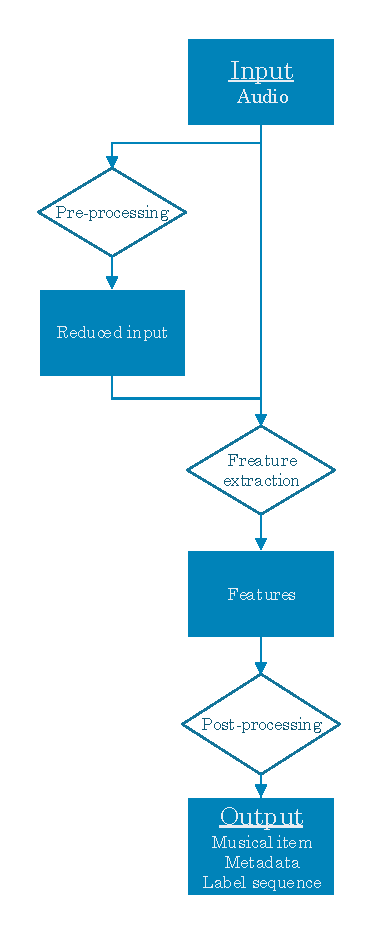
\includegraphics[width = 0.4\linewidth]{obrazky/MIR-diagram.pdf}
    \caption{Řetězec procesů MIR \cite{a_new_companion_to_digital_humanities}}
    \label{fig:MIR_diagram}
\end{figure}

    Digitální hudební nahrávka se jako forma vstupních dat stala hlavním trendem výzkumu \acs{MIR}.
    Je to způsobeno zejména dostupností velkých databází nahrávek ke kterým mají vědecké instituce přístup a nepotýkají se s problémy souvisejícími s autorskými právy \cite{a_new_companion_to_digital_humanities}.

    Z důvodu velké komplexsnosti vstupních dat se využívá několik technik komprimace signálů. 
    Slučování vícekanálových nahrávek do mono sginálu. Převzorkování signálu na nižší vzorkovací kmitočty,
    a rozložení na krátké překrývající se úseky, ze kterých mohou být nezávisle extrahovány jejich vlastnosti\cite{lidy09:448[TUW-181186]}. 
    Výsledkem je kolekce paralelně složených sekvencí hodnot jednotlivých vlastností, které se následně zpracují na požadovaná výstupní data.



    %TODO: Předělat tuhle tabulku
  % \begin{table}[H]
  %   \centering
  %   \begin{tabular}{|p{0.07\linewidth} | p{0.31\linewidth} | p{0.27\linewidth} | p{0.25\linewidth}|}
  %       \hline
  %       {\bf Data}                 & {\bf Vyhledávání informací} & {\bf Klasifikace a odhad} & {\bf Sekvenční značení}\\
  %       \hline
  %       Audio                      & Indetifikace kopie \uv{coverů},
  %                                    Řazení skladeb,
  %                                    Měření podobnosti,
  %                                    Získání otisku,
  %                                    Generování seznamu skladeb
  %                                  & Identifikace umělce a skladatele,
  %                                    Žánr a nálada,
  %                                    Určení tempa
  %                                  & Extrakce melodie,
  %                                    Odhad akordů,
  %                                    Detekce nástupů,
  %                                    Segmentace                   \\
  %       \hline
  %   \end{tabular}
  %   \caption{Typické procesy na základně vstupních a výstupních dat. \cite{a_new_companion_to_digital_humanities}}
  %   \label{tab:MIR_typicke_procesy}
  % \end{table}

  \section{Parametrizace hudebních nahrávek} \label{sec:Parametrizace}
  V této kapitole je popsán audio signál. Jak vzniká, jeho reprezentace v číslicovém zpracování a základní principy práce s audiosignálem.
  V bodech \ref{sec:Dynamika} a \ref{sec:Barva} jsou popsány parametry získávané z audio signálu.
  Získané parametry slouží pro přesnější popis skladby.

  \subsection{Reprezentace audio signálů} \label{sec:Audio}
  Hudební dílo může být reprezentováno více formami.
  Jako tradiční médium pro její ukládání ještě před vznikem záznamu sloužily noty a další typy zápisů pomocí symbolů.
  Výsledné hudební dílo ale představuje mnohem více než počáteční notový zápis.
  Každý hudebník a hudební nástroj do skladby předává svou unikátnost.
  Při hře se noty začnou proměňovat v harmonické zvuky, hladké melodie a nástroje vzájemně rezonují. 
  Každý z hudebníků do skladby přináší svou interptretaci. Jinak reagují na tempo zvýrazňují odlišné noty a liší se jejich artikulace.
  Všechny tyto proměnné ve výsledku způsobují, že dílo není jen mechanické přehrání napsané partitury.
  Jeho součástí se stává unikátní přednes umělce a použitého hudebního nástroje \cite{fundamental_of_music_processing}.

  Z fyzikálního hlediska při interpretaci díla vznikají zvukové vlny šířící se vzduchem.
  Tyto vlny jsou reprezentovány kmítáním částic v pružném prostředí. V takovém prostředí jsou částice na sebe vázány a vytvářejí soustavu oscilátorů. Pokud dojde k vychýlení jedné částice ze své rovnovážné polohy,
  vlivem okolních částic dochází k působení pružných sil a vzniká její kmitání. 
  Zároveň dochází k vzájemnému rozkmitání okolních částit a prostředím se začne šířít vlna. Jednotlivé částice kmitají pouze kolem své rovnovážné polohy. Nedochází tak k přenosu látky ale pouze energie a hybnosti\cite{crocker1998handbook}.
  Popsané kmitání jsme schopní zachytit pomocí akustických měničů.
  Je získán analogový signál šířících se zvukových vln nazývaný jako audio signál.
  Pojmem audio je označován řetězec sloužící k záznamu, přenosu a reprodukci zvuků v mezích lidského slyšení.
  Avšak v audio signálu se už nenachází přesná reprezentace not a jejich paramterů jako jsou čas nástupu, tón, délka trvání, dynamika.
  Díky tomu je analýza hudebních signálů obtížným úkolem a je ovlivněna reprezentací interpreta, stavbou nástroje, akustikou prostoru a vnímáním posluchače.
  Zmíněnými problémy se zabývá samostatný vědní obor s názvem psychoakustika.
  Nejdůležitějšími parametry audio signálu které jsou podrobně popsány níže definujeme: frekvence, výška tónu, dynamika, intenzita, hlasitost a barva \cite{fundamental_of_music_processing}.

  \subsection{Časová oblast}
  Základní reprezentací audio signálu je tzv. zobrazení v \textbf{časové oblasti}.
  V časové oblasti představují číslicový signál vzorky. Jednotlivé vzorky udávají hodnotu signálu v daném čase.
  Počet vzorků vztažených na jednotku času určuje vzorkovací frekvence signálu.
  Důležitým pravidlem pro vzorkování signálu je Shannonův-Nyquistův vzorkovací teorém
  \begin{equation}
    f_{vz} > 2f_{max}
    \label{rov:vzorkovaci_teorem}
  \end{equation}
  kde $f_{vz}$ je vzorkovací frekvence a $f_{max}$ je maximální frekvence v audio signálu \cite{bracewell1978fourier}.  
  Pokud jednotlivé vzorky zobrazíme graficky získáme průběh signálu v čase viz obr.\ref{fig:Waveform}.

  \begin{figure}[H]
    \centering
    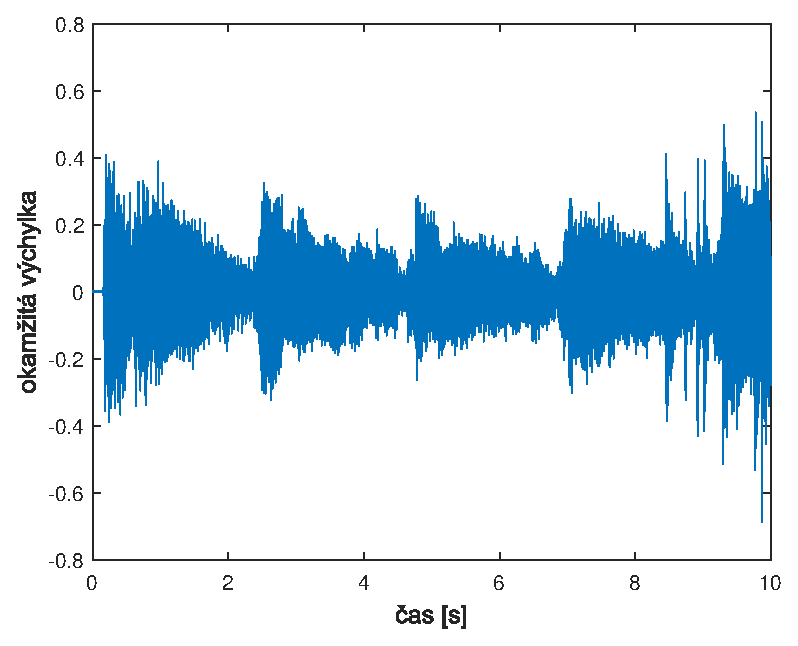
\includegraphics[width = 0.8\linewidth]{obrazky/Waveform.eps}
    \caption{Zobrazení časového průběhu signálu}
    \label{fig:Waveform}
  \end{figure}

  Tato reprezentace audio signálu poskytuje informace o průběhu amplitudy signálu.
  Využívá se například pro výpočet energie signálu popsaný v bodě \ref{sec:Energie_signalu}.
  
  \subsection{Frekvenční oblast} \label{sec:FT}
  Pro získání dalalších informací o hudebním díle se využívá transformace signálu do frekvenční oblasti umožňující odlišné znázornění struktury signálu.

  Ve frekvenční oblasti je signál reprezentován jeho frekvenčními složkami popsanými v komplexním tvaru.
  Spektrum představuje rozložení původní části signálu na jednotlivé frekvenční složky popsané funkcí sinus. Kde reálná složka obsahuje informaci o magnitudě \uv{velikosti} funkce sinus.
  Imaginární složka komplexního čísla pak udává počáteční fázi.
  V grafu jsou poté zobrazeny frekvenční složky se kterých se signál skládá viz obr. \ref{fig:Bass_tone}.


  % \begin{figure}[H]
  %   \centering
  %   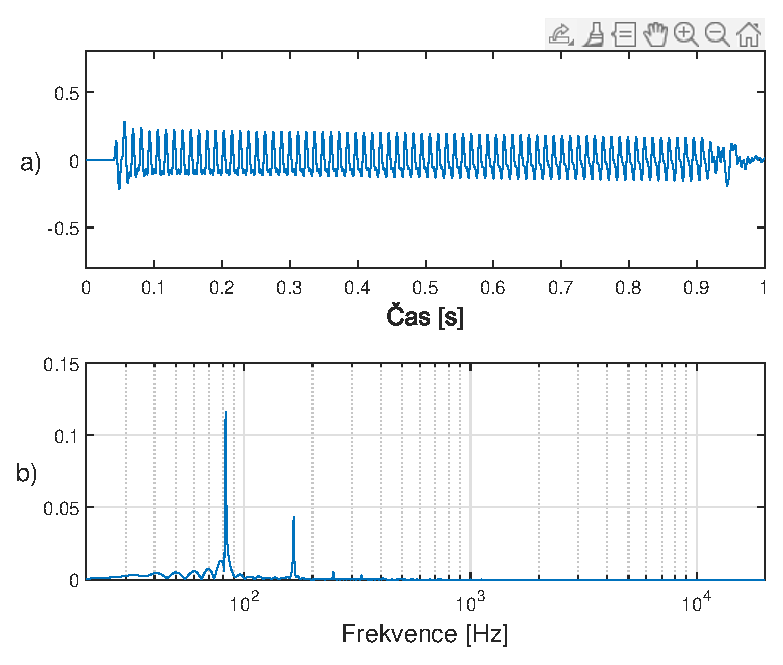
\includegraphics[width = 0.9\linewidth]{obrazky/Bass_tone_spectrum.eps}
  %   \caption{Zobrazení časového průběhu signálu}
  %   \label{fig:Waveform}
  % \end{figure}

  \begin{figure}[H]
    \centering
        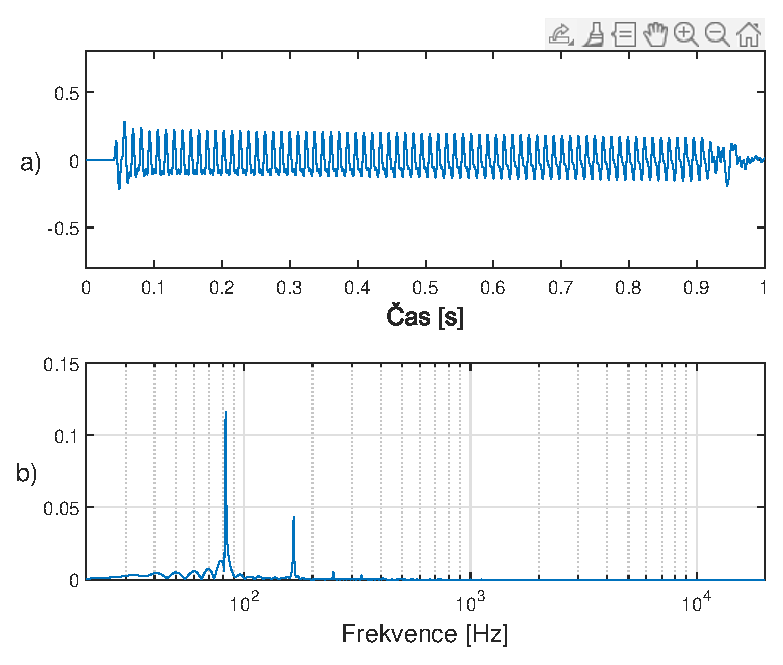
\includegraphics[width = 0.8\linewidth]{obrazky/Bass_tone_spectrum.eps}
    \caption{Reprezentace tónu E zahraného na basovou kytaru. \textbf{a)} Časová oblast ~ ~ ~ ~ ~\textbf{b)} Frekvenční spektrum}
    \label{fig:Bass_tone}
\end{figure}
  
  Jako názorný důvod proč je transformace do frekvenční oblasti přínosná je dán příklad. Na nástroj je zahrán tón, který je zaznamenán. 
  V časové oblasti je možné určit délku tónu a jeho průběh podle ADSR obálky popsané v bodě \ref{sec:Barva}.
  Pokud je ale potřeba zjistit výšku tónu a určit notu, tak se jedná o složýitý proces.
  Díky transformaci do frekveční oblasti je patrná fundementální frekvence tónu.
  Označována také první harmonická.
  Tato frekvence udává výšku tónu a je tak možné stanovit notu která byla zahrána.

  Pro získání frekvenčního spektra signálu je třeba transformovat signál s časové oblasti. K tomu slouží několik úprav Fourierovy transformace podle vlastností vstupního signálu. Tyto metody jsou dále nazývány jako Fourierovy řady, Diskrétní časová Fourierova transformace a Diskrétní Fourierova transformace. V případě audio signálu se vyžívá zejména Diskrétní Fourierovy transformace popsané v bodě \ref{sec:DFT}.

  \textbf{Fourierovy transformace} zkráceně definována jako transformace převádějící signál mezi časovou a fekvenční oblastní poomcí harmonických signálů jež popisují funkce sinus a cosinus \cite{bracewell1978fourier}. Funkce sinus a cosinus představují komplexní exponenciály.
  \begin{equation}
    e^{i\alpha t} = \cos(\alpha t) + i \sin(\alpha t)
  \end{equation}
  Fourierova transformace pro \textbf{ spojitý neperiodický signál} je pak zapsána jako
  \begin{equation}
    X(f) = \int_{-\infty}^{\infty} x(t) e^{-i\omega t} dt
  \end{equation}
  kde $\omega = 2\pi f$ a udává uhlovou frekvenci. Magnituda $|X(f)|$ je potom funkcí sudou \cite{sneddon1995fourier}.

  Pro signál který je \textbf{spojitý a periodický} se definují Fourierovy řady a integrální funkce je počítaná pouze pro jednu periodu signálu
  \begin{equation}
    c[f_k] = \frac{1}{T_0} \int_{0}^{T_0} x(t) e^{-i k \omega_0 t} dt
  \end{equation}
  kde $f_k = k \times f_0$ a $k \in (\mathbb{Z}; 0, \pm 1, \pm 2, \dots)$. Vypočítané spektrum je diskrétní a neperiodické \cite{sneddon1995fourier}.

  Pokud je vstupní signál diskrétní hovoříme o Diskrétní Fourierově transformaci která je více popsána v následujícím bodě \ref{sec:DFT}.

 Po transformaci signálu do frekvenčního spektra jsou data signálu v komplexním tvarua a jejich magnituda $|X(f)|$ je funkce sudá, tím pádem symetrická kolem nuly a fáze $\varphi_x(f)$ je funkcí lichou čili je středově symetrická. Pro analýzu audio signálů se využívá kladná část spektra.

  \subsection{DFT - Diskrétní Fourierova transformace} \label{sec:DFT}

  Pokud jsou signály zpracovávány pomocí výpočetních procesorů,
  tak může být uložen pouze omezený počet hodnot signálu.
  To znamená, že analogový signál spojitý v čase musí být převeden na signál digitální tvz. signál diskrétní, který je není spojitý v čase. 
  Diskrétní signál je potom vhodný pro číslicové zpracování.
  Proto jsou pospsané algoritmy \acs{DFT} přizpůsobené právě pro zpracování diskrétních signálů nespojitých v čase.

  \begin{figure}[H]
    \centering
    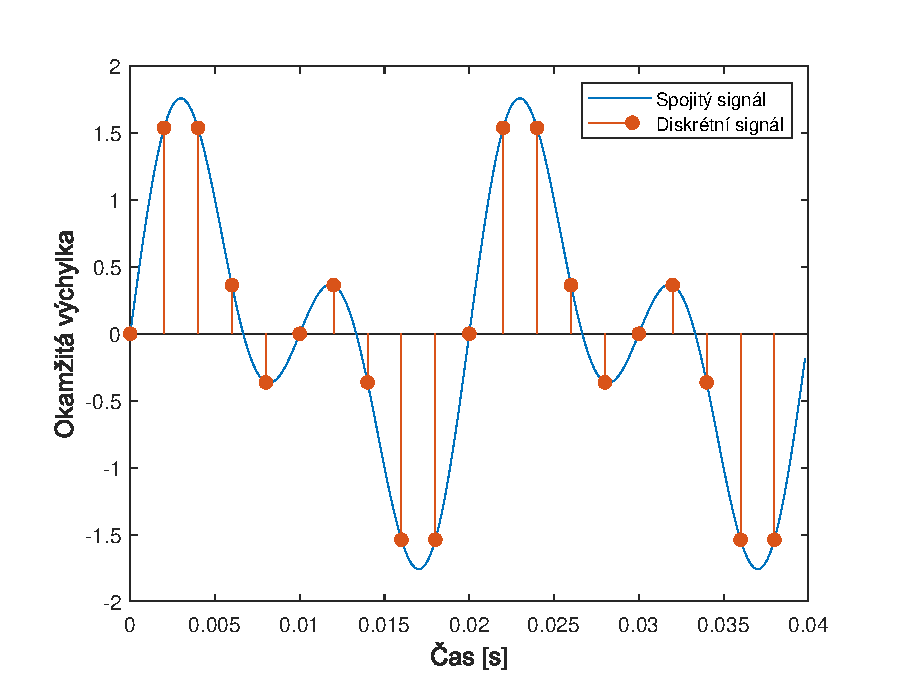
\includegraphics[width = 0.8\linewidth]{obrazky/Discrete_signal.eps}
    \caption{Časově spojitý signál a diskrétní signál}
    \label{fig:Discrete_signal}
  \end{figure}

  Opět jsou dány odlišné definice pro signál diskrétní neperiodický a diskrétní periodický. Protože se jedná o signál diskrétní, tak zde odpadají integrální funkce.
  Pokud se jedná o signál \textbf{diskrétní neperiodický} jeho výsledné spektrum bude spojité a hovoříme o Fourierově transformaci diskrétní v čase. Matematicky je zapsána v následujícím tvaru
  \begin{equation}
    X(f) = \sum_{n = -\infty}^{\infty} x[n] e^{-i \Omega n}
    \label{rov:DTFT}
  \end{equation}
  kde
  \begin{equation}
    \Omega = 2 \pi (f/f_s)
  \end{equation}
  a $f_s$ je vzorkovací frekvence signálu.

  Protože v praxi signál není nikdy nekonečně dlouhý, tak je možné jej poskládat za sebe a vytvořit tak signál periodický. Pro periodické signály je výpočet \acs{DFT} zapsán ve tvaru
  \begin{equation}
    X[f_k] = \sum_{n = 1}^{N_0} x[n] e^{-i\Omega_k n}
    \label{rov:DFT}
  \end{equation}
  kde
  \begin{equation}
    \Omega_k = 2 \pi \frac{f_k}{f_s}
  \end{equation}
  \begin{equation}
    f_k = \frac{k f_s}{N_0}
  \end{equation}
  a $k \in(\mathbb{Z}; 0, N_0 -1)$. $N_0$ udává počet vrzorků v jedné periodě signálu.
  Hustota spektra $K$ v takovém případě odpovídá $K = N_0$.

  Ze strany výpočetní náročnosti je takto definovyný algoritmus neefektivní a výpočetně náročný.
  Pro výpočet \acs{DFT} je zapotřebí velkého množství operací složitost algoritmu je pak zapsána jako $O(N^2)$.
  Proto pokud počet vzorků $N$ dosahuje většího množství je ve spoustě případů tento algoritmus příliš pomalý a neefektivní pro praktické využití.

  Počet potřebných operací může být výrazně redukován. 
  Na vývoj efektivního řešení výpočtu \acs{DFT} se zasloužil Carl Friedrich Gauss a Joseph Fourier zhruba před dvěma sty lety. Tento algoritmus nazýváme Rychlou Fourierovou transformací zkráceně FFT.
  Počet operací pro výpočet takového algoritmu byl snížen na $O(N \log_2 N)$ \cite{fundamental_of_music_processing}.
  Například při použití vzorků $N = 2^{10} = 1024$. \acs{FFT} vyžaduje $N\log_2N = 10240 $ operací namísto $N^2 = 1048576$ operací při použití \acs{DFT}. Jak je vidět snížení výpočetní náročnosti je velké a exponenciálně roste s větším počtem vzorků $N$.
  Vynález \acs{FFT} změnil odvětví zpracování signálů a je dnes využíván v miliardách telekomunikačních zařízeních. Stejně tak i ve zpracování a analýze zvukových signálů hraje důležitou roli \cite{fundamental_of_music_processing}.


  
  \subsection{STFT - Short-time Fourier transform} \label{sec:STFT}

  V roce 1946 Dennis Gabor představil \acs{STFT} jako možnost zařazení frekvenčních složek ke konkrétnímu času signálu \cite{strichartz2003guide}.
  Fourierova transformace umožňovala převod signálu z časové oblasti do frekvenční ale nebylo zřejmé v jakém časovém úseku signálu se získané fekvenční složky nachází.
  Hlavní myšlenkou \acs{STFT} je, že namísto analyzování celého signálu je analyzována pouze jeho malá část.
  Za tímto účelem je definovaná tzv. okénokvá funkce, která je nenulové pouze v malé části signálu.
  Analyzovaný signál je následně vynásoben vzniklou okénkovou funkcí a díky tomu vzniká malá nenulová část signálu dle okénkové funkce viz obr. \ref{fig:STFT}.
  Chceme li analyzovat signál v různých časech je tato funkce po signálu posouvána a následně se počítá \acs{DFT} pro každý výsledný okénkový signál.

  \begin{figure}[H]
    \centering
    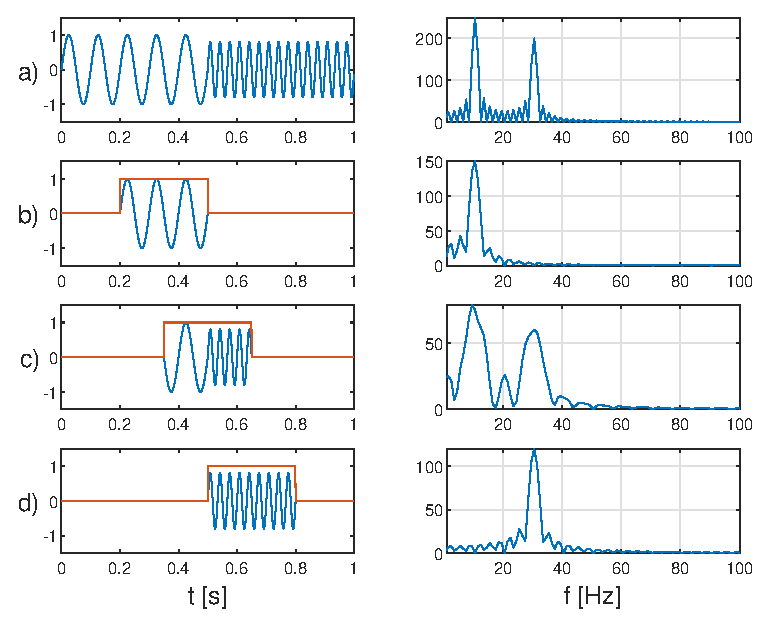
\includegraphics[width = 1\linewidth]{obrazky/STFT.eps}
    \caption{Signál o délce $1 s$ s počáteční frekvencí $10 Hz$ a koncovou frekvencí $30 Hz$ \textbf{a)} Původní signál \textbf{b)} Signál s okénkem od $0,2 s$ do $0,5 s$ \textbf{c)} Signál s okénkem od $0,35 s$ do $0,65 s$ \textbf{d)} Signál s okénkem od $0,5 s$ do $0,8 s$ \cite{fundamental_of_music_processing}}
    \label{fig:STFT}
  \end{figure}

  Na obr. \ref{fig:STFT} je graficky znázorněna myšlenka \acs{STFT}, která ukazuje princip určování frekvenčních složek v čase a jejich výhody. 
  Signál je násoben obdelníkovou okénkovou funkcí ve třech místech.
  Tyto tři vzniklé signály jsou následně na sebe nezávazně transformovány do frekvenční oblasti.
  Z výsledků Fourierovy transformace lze vidět, že každá z těchto částí má jiné frekvenční spektrum.
  Pokud by bylo zapotřebí například určit přesný přechod mezi dvěma frekvencemi nacházejícími se v signálu. Lze zpřesnit časové měřítko analýzy pomocí délky okénka.
  Tím ale dochází ke zmenšení přesnosti ve frekvenční oblasti.
  
  Na výsledku přesnosti analýzy poomcí \acs{STFT} závisí také tvar použité okénkové funkce.
  V obr. \ref{fig:STFT} je použito obdélníkového okénka které díky svým ostrým hranám zkresluje výsledek o nechtěné frekvenční složky.
  Existuje více tvarů okénkových funkcí pro odstranění nežádoucích složek.
  Například to jsou Kaise, Chebyshev, Hann, Haming a další \cite{Time-frequency_distributions}.
  
  Pokud jsou analyzované data skrze okénka funkce \acs{STFT} poskládány zpět za sebe, tak představují matici průběhu frekvenčního spektra signálu v čase.
  Takové zobrazení se nazývá \textbf{spektogram} a v případě 2D zobrazení se skládá z časové a frekvenční osy.
  Magnituda frekvencí je pak zobrazena barevoun škálou. Viz obrázek \ref{fig:Spectrogram}.

  \begin{figure}[H]
    \centering
    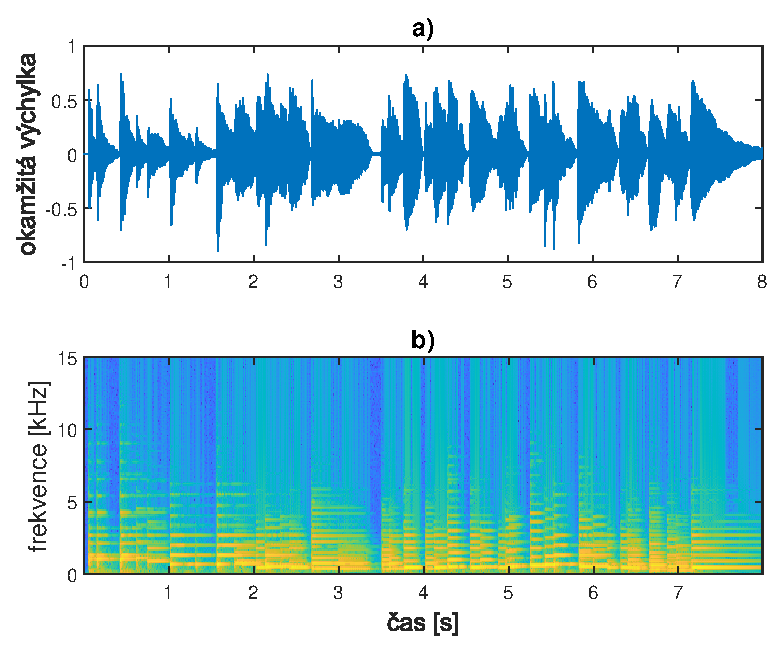
\includegraphics[width = 0.8\linewidth]{obrazky/Spectrogam.eps}
    \caption{Nahrávka piana \textbf{a)} Okamžitý výchylka nahrávky \textbf{b)} Frekvenční spektrum nahrávky zobrazené pomocí spektrogramu}
    \label{fig:Spectrogram}
  \end{figure}

  \subsection{Dynamika hlasitost a intenzita} \label{sec:Dynamika}
  
%TODO: Informace o hlasitosti v češtině MPC-ELE2 přednáška 7 slide 64

  V češtině se pojem hlasitost využívá pro reprezentaci subjektivního vnímání akustického tlaku definovanou například jednotkou phon\footnote{Phon - logaritmická jednotka vyjadřující individuální vnímání hlasitosti. Vnímání hlasitosti lidského ucha je závislé na křivce prahu slyšení a může se lišit pro každý tón \cite{tumarkin_1950}.}. 
  Stejně tak je hlasitost využívána, hovoří li se o měřené hlasitosti vyjádřené například hladinou intenzity zvuku popsanou níže nebo efektivní hodnotou signálu.
  Z důvodu lepší srozumitelnosti jsou dále využívána anglické pojmy \uv{volume} a \uv{loudness}. 
  
  \textbf{Dynamika} popisuje průběh hlasitosti \uv{volume}interpretovaného hudebního díla. Udává jeden z faktorů jak lze například odlišit stejnou skladbu zahranou různými muzikanty. Interpretací skladby umělec vytváří dynamiku přednášeného díla \cite{fundamental_of_music_processing}.
  V notovém zápise je dynamika neboli hlasitost přednesu popsána symboly jako jsou například pianissimo \uv{\emph{pp}}, piano \uv{\emph{p}}, forte \uv{\emph{f}} a další.

  V audio signálu je dynamika brána jako hlasitost \uv{loudness} Jedná se o změny apmlitudy signálu nebo jeho efektivní hodnoty \acs{RMS}\footnote{RMS - udává statistickou hodnotu z měření velikosti veličin. Je využívána u periodických veličin\cite{RMS_value}.} v čase.

  Při měření hlasitosi \uv{loudness} v akustickém prosotru je pak využíváno pojmů \textbf{intenzita} zvuku a \textbf{akustický výkon}.
  Akustický výkon je definovánjako množství energie  vyzářené akustickým vysílačem ve vzduchu za jednotku času.\cite{acoustic_power}. Jednotkou je $W$.
  A intenzita zvuku je pak definována jako množství energie, které projde jednotkovou plochou kolmou na směr šíření na jednotku času. Jednotkou je $Wm^{-2}$ \cite{intenzita_zvuku_definice}
  
  Z pohledu vnímání hlasitosti lidským uchem je rozsah vnímané intenzity zvuku v řádech bilionů. Práh slyšení činí $10^{-12}$ $Wm^{-2}$ a práh bolesti je $10$ $Wm^{-2}$.
  Pro zmenšení tak velkého řádu je definována hladina intenzity zuvku v decibelech $dB$. Kde vztažnou hodnotou je práh slyšení $I_0 = 10^{-12}$ $Wm^{-2}$.
  Hladina intenzity se vypočítá dle rovnice \ref{rov:hladina_intenzity}.

  \begin{equation}
    L_I = 10log(\frac{I}{I_0})
    \label{rov:hladina_intenzity}
  \end{equation}

  \subsection{Barva} \label{sec:Barva}

  V hudebním vyjádření se za slovem barva zkrývá komplexní sdružení atributů.
  Jedná se jak o psychologický tak hudební problém, který je vnímán individuálně\cite{The_perception_of_musical_timbre}.

  Zjednodušeně se barva definuje jako vlastnosti, díky kterým je možné rozeznat tón o stejné výšce a hlasitosti zahraný na dva různé náastroje\cite{MULLER2014713}.
  Díky barvě je posluchač schopen rozeznávat odlišné zvuky nástrojů a typů interpretace.

  Z důvodu špatné kategorizace barvy fyzikálními veličinami je většinou interpretována přídavnými jmény.
  Například je barva popisována jako jasná, temná, ostrá, čistá, teplá, pestrá, nazální, tonální a další.

  Jedním z možných nástrojů pro analýzu barvy tónu je tvz. obálka tónu \uv{signálu}.
  Obálku určuje okamžitá výchylka signálu v čase viz obr. \ref{fig:ADSR_envelope_on_piano_tone}
  Je rozdělena na 4 fáze popsané z knihy Fundamentals of Music Processing \cite{fundamental_of_music_processing}.
  \textbf{Attack \uv{náběh}} určující začátek tónu. Například úder paličkou na blánu bubnu.
  V této fázi se nachází více ruchových složek z daného úderu a má velkou dynamiku.
  Následuje fáze s názvem \textbf{Decay \uv{útlum}}.
  Po hlasitém úderu okamžitá výchylka signálu klesá a začíná převládat tonální složka. Decay udává dobu za kterou se signál z jeho maxima sníží na hodnotu sustain.
  \textbf{Sustain \uv{podržení}} je fáze ve které je zřetelný tón a stálá hlasitost. Rezonující blána bubnu.
  Poslední fází je \textbf{Release \uv{uvolnění}} při kterám dochází k poklesu hlasitosti zdroje zvuku až k uplnému utlumení.
  Například přiložení tlumítka na rezonující strunu.

  \begin{figure}[H]
    \centering
    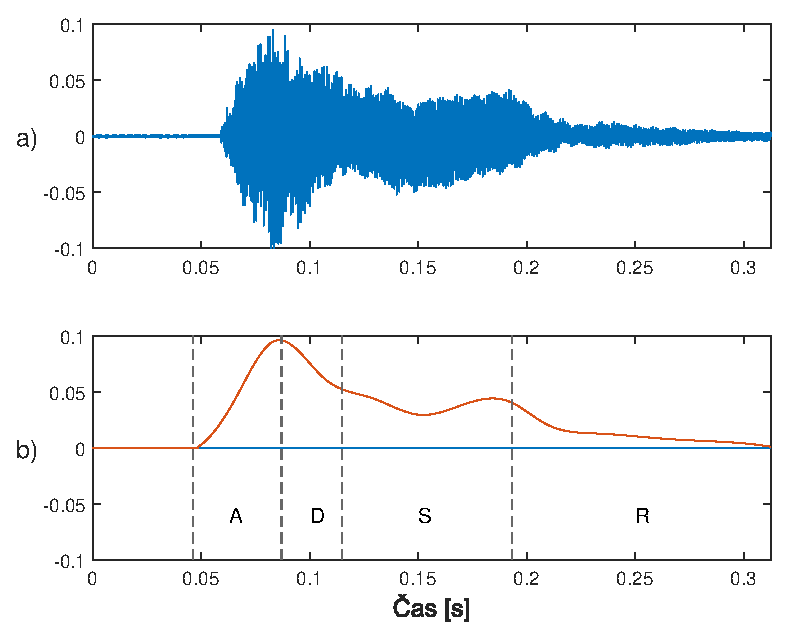
\includegraphics[width = 0.8\linewidth]{obrazky/ADSR.eps}
    \caption{Tón A5 zahraný na klavír \textbf{a)} Okamžitá výchylka tónu \textbf{b)} ADSR obálka tónu}
    \label{fig:ADSR_envelope_on_piano_tone}
  \end{figure}

  Další informace o barvě signálu se nacházejí v jeho frekvenčním spektru. 
  Tón zahraný na hudební nástroj má svou fundamentální \uv{nosnou} frekvenci nazývanou první harmonická udávající jeho výšku.
  Dle konstrukce nástroje se v signálu objevují násobky nosné frekvence.
  Tyto násobky představují vyšší harmonické složky tónu.
  Počet a amplituda vyšších harmonických složek má vliv na výslednou barvu tónu a je to hlavní důvod proč je lidské ucho schopné rozeznat stejný tón znějící na různé nástroje. %TODO: Bylo by vhodné poslední větu ocitovat.

  %TODO: vložit obrázek spektrogramu tónu

\section{Detekce nástupů a analýza tempa skladby} \label{sec:Detekce_tempa}
% V této kapitole jsou posány principy analýzy tempa skladby a detekce dob sklady. 
S vývojem nových technologií se mění i přístupy využívané v \acs{MIR} pro analýzu tempa skladby. 
V této kapitole je popsán postupný vývoj algoritmů.
Od nejjednodušších přístupů po komplexní řešení využívající moderní metody hlubokých neuronových sítí.

Detekce nástupů lze chápat jako detekci začátků not či dalších hudebních událostí, které se vyskytnou v průběhu skaldby.
Výskyt takových udáslotí je provázen zvýšením energie signálu zaznamenané ve fázi nástupu dle ADSR obálky popsané v bodě \ref{sec:Barva}.
Typickým znakem pro fázi nástupu je rychlý nárůst obálky amplitudy signálu.
V této fázi se při vytváření tónu vyskytují \textbf{Tranzienty}. Tranzienty je možné pozorovat zejména u neperkusivních nástrojů například u dechových nebo smyčcových.
Jsou představovány nakmitávajícími a dokmitávajícími pochody. Jedná se o zvuk netónové podoby připomínající hluk s výraznými frekvenčními změnami.
U smyčcových nástrojů takový zvuk může být ze začátku způsoben drhnutím smyčce o strunu do chvíle než se ustálí její kmitání. Délka tranzientů pak může dosahovat od jednotek milisekund až po stovky milisekund v závisloti na typu nástroje a technice hry \cite{syrový2013hudební}.
Například v případě piana tranzient odpovídá počáteční fázi kdy byla zmáčknuta klávesa.
Na základě zmáčknutí klávesy dochází ke zvednutí tlumítka, kladívko udeří do struny, struna začíná vibrovat a vibrace se přenáší do těla piana.
V této fázi začíná tělo rezonovat a konečně dochází k ustálení tónové složky. Při úderu kladívka dochází k velkému přenosu energie patrném na obálce tónu. Díky tomu je lehké určit začátek tónu podle nárůstu amplitudy obálky \cite{fundamental_of_music_processing}.

U některých nástrojů je však energie přenášená po celou dobu znění tónu konstantně a dochází k pomalému jemnému náběhu tónu například u určitých technik hry na smyčcové nástroje nebo u dechových nástrojů. Fáze náběhu je pak pomalá a dlouhá a plynule přechází do fáze podržení. Pro tyto jemné zvuky se stává obtížné určit skutečnou pozici začátku noty.

%TODO: doplnit obrázek obálka perkusivního zvuku a táhlého



Náročnost detekce nástupů se zvyšuje v případě, že nehraje pouze jeden nástroj. Jedná se například o polyfoní skladbu. Polyfoní skladbou rozumíme skladbu tvořenou více hlasy.
Zároveň nemají určenou roli vedoucího a doprovodného hlasu \cite{6155601}.
Takové uspořádání hlasů může vést k překrývání a nástupy mohou být maskovány. Díky jevu maskování je obtížné zaznamenat změny energie signálu. V tomto případě přichází potřeba po komplexnějších metodách detekce nástupů \cite{fundamental_of_music_processing}. Například pohled na krátkodobé změny ve spektru signálu pomocí využití \acs{STFT} popsané v bodě \ref{sec:STFT}.

  \subsection{Využití energie signálu} \label{sec:Energie_signalu}

  Jak již bylo zmíněno při hraní dochází k přenosu energie od hřáče na hudební nástroj.
  Tento přenos je ve značné míře provázen rychlým nárůstem amplitudy ve fázi náběhu na začátku tónu.
  Například při úderu kladívka piana na strunu nebo úderu paličky na blánu bubnu.
  Ná základě tohoto jevu je možnost detekovat nástup tónu pomocí funkce pro výpočet energie signálu v daném místě.
  Náhlé změny signálu v takto definované funkci ukazují potencionální místa nástupů.
  Matematicky pak funkci popisujeme. 
  Stejně jako u \acs{STFT} popsané v bodě \ref{sec:STFT} je definována okénková funkce $w(n)$ ve tvaru zvonu \uv{bell-shaped function} která je posouvaná po diskrétním signálu $x(n)$.
  Okénková funkce je symetrická podle počátku a potom platí že $ m \in [-M : M]$ a $M \in \mathbb{N}$. Funkce lokální energie signálu je pak zapsána
  \begin{equation}
    E_{xw}(n) = \sum_{m = -M}^{M} |s(n+m)w(m)|^2
  \end{equation}
  pro $n \in \mathbb{Z}$ \cite{fundamental_of_music_processing}.

  \begin{figure}[H]
    \centering
    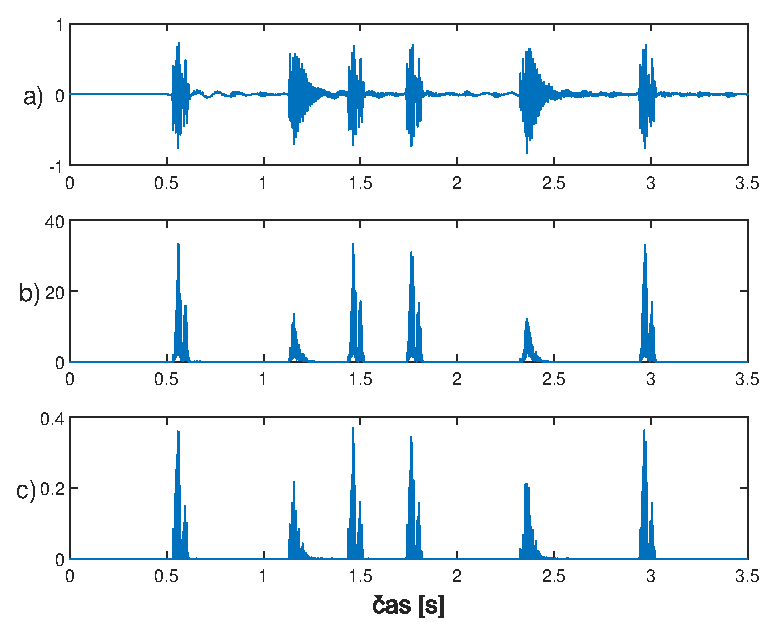
\includegraphics[width = 0.8\linewidth]{obrazky/Energy_based_novely.eps}
    \caption{Detkte nástupů perikusivního zvuku \textbf{a)} Okamžitá výchylka nahrávky \textbf{b)} Lokální energie signálu $E_{xw}(n)$ \textbf{c)} Derivace lokální enegrie signálu s půlvlnným usměrněním $\Delta_E(n)$}
    \label{fig:energy_based_novelty}
  \end{figure}

  Pro názornější zobrazení se následně vypočítá derivace funkce lokální energie. V případě diskrétního signálu se derivace realizuje jako rozdíl dvou po sobě jdoucích vzorků. Protože pro detekci nástupů je důležitá zejména pozitivní změna energie nikoliv její pokles jsou ponechány pouze pozitivní rozdíly a negativní jsou zapsány jako nulové. V anglické literatuře je tneto proces známý také jako půlvlnné usměrnění \uv{half-wave rectification}. Vzorce jsou zapsány následovně 
  \begin{equation}
    r = E_{wx}(n+1) - E_{wx}(n)
  \end{equation}
  \begin{equation}
    \Delta_E(n) = \frac{r + |r|}{2} = \genfrac{\lbrace}{}{0pt}{}{r, \; \text{if} \: r \geq 0 }{0,\; \text{if} \: r < 0}
  \end{equation}
  kde $r \in \mathbb{R}$ a $n \in \mathbb{Z}$.
  Na obr. \ref{fig:energy_based_novelty} lze vidět zobrazení takto vypočítané lokální energie signálu a její derivace. Analyzovaný signál se skládá z několika perkusivních úderů.
  Pro výpočet bylo použito okno typu \uv{bell-shaped function} o velikosti 201 vzorků.


  \subsection{Využití spektra signálu}

  Díky rozložení signálu na jeho spektrum pomocí Fourierovy transformace popsané v bodě \ref{sec:FT} je možné lépe rozeznat strukturu nahrávky a zmírnit efekt maskování který nastává při metodách založených na energii signálu popsaných v bodě \ref{sec:Energie_signalu}.
  V polyfonní hudbě mohou interpretace o nižší hlasistosti bý maskovány hlasitějšími projevy.
  Kdy například jeden nástroj v tónové fázi podržení ADSR obálky, popsané v bodě \ref{sec:Barva}, může být hlasitější než fáza náběhu druhého nástroje.
  Takový nástup je pak maskován a je obtížná jeho detekce.
  V případě maskování některých z nástrojů v časové oblasti je možné spektrum signálu zaměřit na frekvenční oblast spektra ve které se maskovaný nástroj nachází.
  Díky tomu je možné nástup tónu takového nástroje detekovat pomocí spektra signálu. Každý hudební nástroj obsahuje jiné frekvenční spektrum \cite{fundamental_of_music_processing}.
  Díky tomu se různé nástroje nachází na odlišných místech spektra, jak spektrum daného nástroje vypadá určuje také barvu popsanou v bodě \ref{sec:Barva}.
  S takovým jevem je důležité počítat při detekci nástupů založené na spektru signálu. 
 
  Jedním ze spůsobů analýzy nástupů pomocí spektra je detekovat změny ve spektru v průběhu času. Při zobrazení časového průběhu spektra nazývaného spektogram popsaný v bodě \ref{sec:STFT}.
  Jsou za sebou v čase poskládány vektory nesoucí informaci o spektru.
  Pokud jsou počítány rozdíly mezi dvěma po sobě jdoucími vektory spektogramu jsou získány informace o změně spektra v čase.
  Protože tranzienty se při fázi náběhu skládají z části z ruchové složky rozléhající se přes velkou část slyšitelného frekvenčního spektra je tak možné detekovat nástupy.
  Popsané metodě porovnávání vektorů se také říká \textbf{spektrální tok} \cite{fundamental_of_music_processing}.
  Pro výpočet spektrálního toku existuje více druhů přístupů lišících se předszpracováním dat a konečným zpracováním výsledků.
  Níže jsou popsány dvě metody výpočtu ze spektogramu a náslezdně z mel spektogramu.

  Výpočet spektrálního toku se provede derivací vstupního diskréntího signálu který zde představuje vektory spektrálních složek. Výpočet probíhá pro každou spektrální složku a výsledek je sečten. Popsáno rovnicí 
\begin{equation}
  r(n) = \sum_{k = 0}^{K} |X|(n+1,k) - |X|(n,k)
\end{equation}

\begin{equation}
  \Delta S_t(n) = \frac{r(n) + |r(n)|}{2} = \genfrac{\lbrace}{}{0pt}{}{r, \; \text{if} \: r \geq 0 }{0,\; \text{if} \: r < 0}
\end{equation}
  kde $ n \in \mathbb{Z}$ a $K$ je počet spektrálních složek v jednom vektoru.
  \begin{figure}[H]
    \centering
    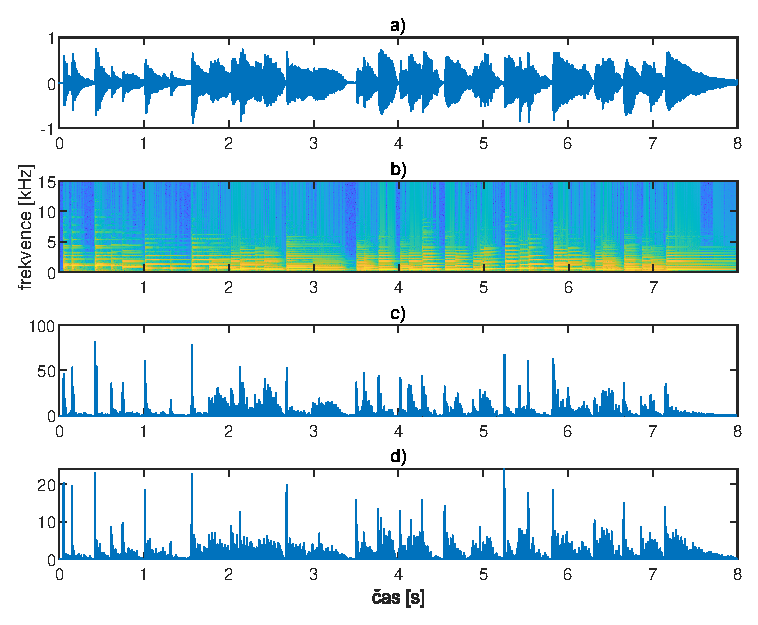
\includegraphics[width = 0.9\linewidth]{obrazky/Spektralni_tok.eps}
    \caption{Výpočet spektrálního toku pro nahrávku piana \textbf{a)} Okamžitá výchylka nahrávky \textbf{b)} Spektogram narhávky \textbf{c)} Spektrální tok bez komprese \textbf{d)} Spektrální tok s kompresí spektra $\gamma = 1$}
    \label{fig:Spectralni_tok}
  \end{figure}
  Pro dosažení přesnějších výsledků je možnost komprese spektrogramu. Funkce pro logaritmickou kompresi singálu je zapsána jako 
  \begin{equation}
    X_c = \log (1+\gamma |X|)
  \end{equation}
  kde pro správnou kompresi je pottřeba aby $\gamma \geq 1$.
  Míra komprese je určena velikostí $\gamma$. Nižší hodnoty jsou vhodné pro lepší detekci perkusivních zvuků.
  Při vyšších hodnotách $\gamma$ dochází k větší kompresi spektrogramu a jsou zřetelnější zvuky o nižší intenzitě.
  Při velké kompresi dochází také k zvýraznění ruchových složek signálu \cite{fundamental_of_music_processing}. 


  Například v článku z \acs{ISMIR} 2021 \cite{tempobeatdownbeat:book} je spektrální tok počítán s Mel Spectogramu popsaného níže.
  Protože lidské ucho vnímá výšku frekvence logaritmicky je jednodužší rozeznat rozdíl mezi frekvencemi u nižší části spektra než u vyšších frekvencí.
  Například rozdíl mezi 500 Hz a 1 kHz je pro lidské ucho dobře detekovatelný a zřetelný.
  Odlišné rozlišovací schopnosti výšky v různých frekvenčních pásmech je způsobeno biologickým rozvržením vnitřního ucha. Proto pro lepší rozlišování na základě lidského vnímání zvuku vznikla Melova stupnice.
  \textbf{Melova stuopnice} je vjemová škála výšek, které posluchač posoudil jako od sebe stejně vzdálené. Referenčním bodem je pak definováno 1000 mel které odpovídají frekvenci 1000 Hz\cite{StevensS.S1937ASft}.
  Výpočet spektrálního toku je následně stejný jak pří výpočtu ze spektogramu. Výslednou křivku je možné vidět na obr. \ref{fig:Mel_spectralni_tok}.

  \begin{figure}[H]
    \centering
    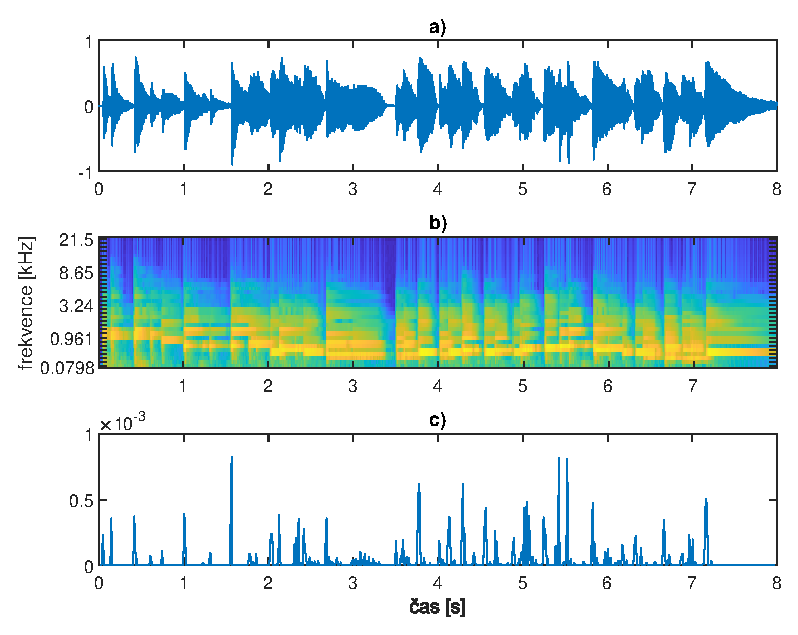
\includegraphics[width = 0.8\linewidth]{obrazky/Mel_spektralni_tok.eps}
    \caption{Výpočet spektrálního toku z mel spektrogramu pro nahrávku piana \textbf{a)} Okamžitá výchylka nahrávky \textbf{b)} Mel spektogram narhávky \textbf{c)} Spektrální tok}
    \label{fig:Mel_spectralni_tok}
  \end{figure}

  % Možnností postprocesignu je například výsledný spektrální tok proložit funkcí lokálního průběmru
  % \begin{equation}
  %   \mu(n) = \frac{1}{2M + 1} \sum_{m = -M}^{M} \Delta S_t(n + m)
  % \end{equation}

  \subsection{Detekce periodicity}
    Detekce periodicity je nezbytnou součástí procesu při detekci dob skladby.
    Důležitou technikou pro detekci periodicity je autokorelační funkce.
    Autokorelační funkce slouží pro detekci periodických vzorů v datech.
    Tato metoda dokáže detekovat tempo, ale neumožňuje určit o jakou dobu se jedná.
    Základní použití je výpočet autokorelační funkce s energie signálu z bodu \ref{sec:Energie_signalu}. Matameticky je pak popsána dle rovnice \ref{rov:autocorelation}. \cite{Signal_processing_methods_for_music_transcription}

    \begin{equation}
      r(n,i) = \sum_{u = -(T_w / 2) + 1}^{T_w / 2} E(n+u)E(n+u-i)
      \label{rov:autocorelation}
    \end{equation}

    Při detekci periodicity je možné využít také banky rezonátorů hřebenového filtru s konstantním poločasem \cite{Tempo_and_beat_analysis_of_acoustic_musical_signals} nebo fázově blokující rezonátory \cite{Resonance_and_the_perciption_of_musical_meter}.


    Autokorelačn funkce zde přináší několik výhod. Jednoduchost a efektivita. Je to jednoduchá metoda pro zjisštění periodicity v signálech a vyžaduje menší množství paměti než jiné víše zmíněné metody. Autokorelace může odhali ne zcela zřejmé periodické vzory, které nemusí být při poslechu nebo pozorování okamžitě zřejmé. Zároveň je robustní vůči šumu. Při analýze také nedochází ke ztrátě informace. \cite{Tempo_and_metrical_analzsis_by_tracking_multiple_metrical_levels_using_autocorrelation}
    
    Autokorelace má také své nevýhody. Není vhodná pro analýzu v reláném čase protože potřebuje dostatečné množství dat a je potřebné aby v analyzovaném datovém okně byla obsažena celá perioda. V opačném případě nedojdte k jejímu nalezení. Autokorelace není schopná pracovat s fází signálu. Pro rozpoznání fáze je zapotřebí dalších metoda. Nekonstantní tempo v analyzovaném signálu představuje pro autokorelační analýzu problém.\cite{Tempo_and_metrical_analzsis_by_tracking_multiple_metrical_levels_using_autocorrelation}

    %TODO: popsat autokorelační funkci a její využití pro detekci tempa (periodicity)

  % \subsection{Vzužití neuronových sítí}  -----Zatím přeskakuju než najdu vhodné zdroje---
  %   Deep neural networks(DNN)
    %TODO: popsat dep learnin při beat trackingu https://tempo beatdownbeat.github.io/tutorial/ch3_going_deep/overview.html
    %TODO: popsat postup (preprocessing, DNN, post processing)/(feature extraction, likelihood estimation, post processing)
  
  % \subsection{Více vrstvé perceptronové sítě}

  % \subsection{Konvoluční neuronové sítě}
  %   Temporal Convolutional networks

  % \subsection{Rekurentní neuronové sítě}
  %   Gated recurent units
  %   Bi-directional models

  % \subsection{Hybridní architektury}

\section{Klasifikace žánrů a nálady} \label{sec:Klasifikace_zanru}

% https://dspace.cvut.cz/bitstream/handle/10467/65310/F3-BP-2016-Bartos-Jaroslav-detekce_hudebnich_zanru_pro_ucely_masteringu_gramofonovych_desek.pdf?sequence=1&isAllowed=y

\section{Chromavektory} \label{sec:Chroma_vektory}

\section{Dostupná řešení} \label{sec:Dostupna_reseni}
    Díky věděcké základně v oblasti music infromation retrieval vznikají open source knihovny umožňující snadné použití v programovacím jazyce python. Tyto knihovny jsou šířeny za účelem usnadnění práce v oblasti \acs{MIR}. Cílem některých knihoven je usnadnit přechod výzkumných týmů do programového jazyka Python a zakomponovat moderní praktiky softwarového vývoje. Díky tomu se staly tyto metody dostupné širší komunitě vědců.\cite{Librosa} V této kapitole je popsáno několik rozšířených knihoven poskytující metody z oblasti \acs{MIR}.

\subsection{Librosa} \label{sec:Librosa}
    Knihovna Librosa vznikla v roce 2015 na základě potřeb vědecké komunity pro snadné použití metod z oblasti \acs{MIR} v jayzce python.
    Publikován a popsána byla článkem Audio and Music Signal Analysis in Python \cite{Librosa} na SciPy 2015.
    Jedná se o otevřenou knihovnu jejiž další vývoj probíhá zapomoci vědecké komunity na GitHubu kde je kladen důraz na kompatibilitu, řádnou dokumentaci obsahující popisy funkcí s příkladovými kódy, a testování funkčnosti. Knihovna obsahuje pokročilé metody pro detekci dob.

    Librosa obsahuje funkce pro extrakci audio vlastností.
    Pro tuto práci jsou důležitými funkcemi zejména Detekce tempa a dob skladby, rozpoznání začátků tónů. Následně jsou v knihovně obsaženy nástroje pro vizualizaci získaných vlastností. Například zobrazerní spektrograma či grtafické zobrazení detekovaného tempa a dob.
    Funkce pro detekci tempa a dob skladby pomocí dynamického programování je v knihovně zapsána:

    \begin{lstlisting}
      tempo, beats = librosa.beat.beat_track(y=y, sr=sr)
    \end{lstlisting}
    
    Kde $ y $ je analyzovaný signál a $ sr $ je vzorkovací frekvence signálu.
    Detekce dob je ve funkci $ brat_track() $ realizována pomocí dynamického programování. Proces je rozdělen na 3 etapy popsané Danielem P.W. Ellis ve článku Beat Tracking by Dynamic Programing \cite{Beat_tracking_by_dynamic_programing}. Jedná se o tyto kroky:

    \smallskip

    \begin{enumerate}
      \item Výpočet obálky síly nástupů
      \item Globální odhat tempa
      \item Porovnání obálky síly nástupů s globálním tempem
    \end{enumerate}

    \smallskip

    \begin{description}
      \item[Výpočet obálky síly nástupů:] Při výpočtu obálky síly nástupů je vstupní sighnál převzorkován na 8 kHz. Poté je vypočítána \acs{STFT} s délkou okna 32 ms a 4 ms mezerou mezi okny. Vypočítaný spektogram je převeden na mel spektrogram o 40 mel pásmech. Mel stupnice je využívána ve snaze vyrovnat důležitost každého frekvenčního pásma v návaznosti na logaritmické vnímání frekvencí lidským uchem. Mel spektogram je převeden na dB a následně jsu počítány diferenciální rovnice prvního řádu podle času pro každé mel pásmo. Principem půlvnlného usměrnění jsou výsledné negativní hotnoty změněny na nulové. Hodnot kladné jsou v daném čase sečteny napříč všemi pásmy. Výsledný signál je filtrován horní propustí s mezní frekvencí 0,4 Hz a vyhlazen pomocí konvoluce s Gaussovy obálky s šířkou okolo 20 ms. Pomocí výše popsaného procesu je získána jednorozměrná obálka síly nástupů v závislosti na čase reprezentující proporcionální nárůst energie přibližně sečtené ve mel pásmech.
      \item[Globální odhad tempa:] Globální odhad tempa je určen z obálky síly signálu $O(t)$ získané v předchozím kroku. Je počítána autokorelace mezi původní obálkou signálu $O(t)$ a jejími zpožděnými verzemi. Pro zpoždění ve kterých se potká velké množství vrcholů obálky nastává velká korelace. Tato korelace může nastat v celočíselných násobcích dané hodnoty zpoždění. Díky tomuto jevu je těžké určit který čas zpozdění představuje správné tempo skladby. Avšak lidmi vnímané tempo skladeb má sklon být kolem 120 \acs{BPM} jak bylo zjištěno ve výzkumu popsaném v článku Ambiguity in Tempo Perception: What Draws Listeners to Different Metrical Levels? \cite{Ambiguity_in_tempo_perception}. Proto je na výslednou autokorelaci aplikováno váhové okno snižující hodnotu autokorelace se vzdáleností od 120 BPM. Čas ve kterém autokorelace dosahuje největší hodnoty je čas hledaného tempa skladby.  
      \item[Porovnání obálky síly nástupů s globálním tempem:] Matematicky je tento krok fomulován rovnicí \ref{rov:Dynamic_programing_formula_for_beat_tracking} kde $ \{t_i\} $ je pole nalezených dob, $O(t)$ je obálka síly signálu, $\alpha$ je váhový koeficient určující důležitost mezi obálkou síly signálu a detekovaným tempem. Funkce $F(\Delta t, \tau_p)$ zapsaná rovnicí \ref{rov:actual_vs_ideal_time_spacing} měří konzistenci mezi skutečným časem od sebe vzdálených dob $\Delta t$ a ideálním časem mezi dobami $ \tau_p$ určeným cílovým tempem.

      \begin{equation}
        C(\{t_i\}) = \sum_{i = 1}^{N} O(t_i) + \alpha \sum_{i = 2}^{N} F(t_i - t_{i-1}, \tau_p)
        \label{rov:Dynamic_programing_formula_for_beat_tracking}
      \end{equation}
  
      \begin{equation}
        F(\Delta t, \tau) = -(log \frac{\Delta t}{\tau})^2
        \label{rov:actual_vs_ideal_time_spacing}
      \end{equation}
    \end{description}
    
\subsection{Madmom}
\subsection{Aubio}
\subsection{Hodnocení extrakce informací} \label{sec:Mir_eval}

\section{Systém Spectoda} \label{sec:Spectoda}

Systém Spectoda je vytvořen a spravován společností Light Seekres s.r.o. sýdlící v Praze. Spectodu představují jako nový komunikační protokol pro bezdrátové ovládání světelncýh produktů \cite{Spectoda}. Pro převod digitálních příkazů v podobě Spectodakódu na světelné animace je využíváno procesorů ESP32 a jeich varianty umístěné ve vlastních obvodech speciálně navržených pro různé problematiky využití. 

Spectoda kód představující animaci je zároveň uložen na plošené desce. Proto v případě ztráty signálu se zdrojem kódu, může světelné zařízení nadále pracovat. Tím se systém stává výhodnější oproti rozšířenému protokolu DMX\footnote{Digital Multiplexer - Protokol pro digitální přenos informací a řízení scénických světel \cite{DMX}.}, u kterého je nutný nepřetržitý tok příkazů. 

Systém spectoda využívá pro generování animací několik základní animací. Tyto animace následně mohou být mezi sebou odčítány sčítány a skládány do bloků animací. Animace i bloky je možné posouvat a skládat zasebe či přes sebe v čase.
 
%\section{Hudební signál jako animace}